\documentclass[a4paper,12pt]{report}
\usepackage{amsmath}
\usepackage{subcaption}
\usepackage[utf8]{inputenc}
\usepackage[T1]{fontenc}
\usepackage{xcolor,graphicx}
\usepackage[top=0.6in,bottom=0.6in,right=1in,left=1in]{geometry}


\begin{document}
\begin{titlepage}
    % \pagecolor{blue!10}
    \begin{center}
        \begin{minipage}{2.5cm}
        \begin{center}
            
\includegraphics[width=2.3cm,height=2.5cm]{slogan.jpg}
        \end{center}
    \end{minipage}\hfill
    \begin{minipage}{10cm}
        \begin{center}
      {\bfseries\large Cairo University - Faculty of Engineering}\\[0.1cm]
      {\bfseries\large Computer Engineering Department}\\[0.1cm]
      \end{center}
    
    \end{minipage}\hfill
    \begin{minipage}{2.5cm}
        \begin{center}
            
\includegraphics[width=2.5cm,height=2cm]{logo_cufe.png}
        \end{center}
    
    \end{minipage}
    
    \vspace{5cm}
    
    {\Huge \bfseries \uppercase{M-ary Amplitiude Shift Modulation} \\[0.5cm] }
    {\LARGE \bfseries Subject: Digital Communication}
    \textsc{\Large }\\[1cm]
    
    \vspace{5cm}
    
    % Author and supervisor
    \begin{minipage}{15cm}
      \begin{flushleft} \huge
        \emph{Submitted to:}\\
        Dr.~Mai \textsc{Badawi}\\
      \end{flushleft}
    \end{minipage}
    
    \vspace{2cm}
    
    
    {\huge \textit{Presented by: }}\\[0.5cm]
    
    \color{black}
    \centering
    \begin{tabular}{lll}
    \large Evram \textsc{Youssef} : & \large Sec: 1 & \large BN: 9 \\[0.1cm]
    
    \end{tabular}
    
    \vfill
    
    % Bottom of the page
    {\LARGE {Year}\\ 2019/2020}
    \end{center}
    \end{titlepage}

% This can be done by adding the \pagenumbering{gobble}
% command and then changing it back to \pagenumbering{arabic} 
% on the next page numbers like so:
    \pagenumbering{gobble}
    \newpage
    \pagenumbering{arabic}

    \pagenumbering{gobble}
    \tableofcontents
    \listoffigures
    \listoftables
    \newpage
    \pagenumbering{arabic}

% These commands for Sectioning...
% The section commands are numbered and will appear in the table of contents of your document.
% Paragraphs aren't numbered and won't show in the table of contents.
    % \section{}
    % \subsection{}
    % \subsubsection{}

    % \paragraph{}
    % \subparagraph{}
%EXAMPLE
    \section{Part 1}
        Digital Communication

    \subsection{Problem 1}
        Figure 1 below showing the comparison between simulated BER and theoritical (analytical) BER
        VS the Eb/N0 in db.

        Please notice, you'll have to input the no. 
            of bits you wish to be transmitted, and it has to be divisible by 3.
    \subsection{Problem 2}
        The constellation of the 8-ary with decision region pf each symbol.
        \begin{figure}[h!]
            %I put \linewidth into the brackets, which means the picture will be scaled to fit the width of the document.
            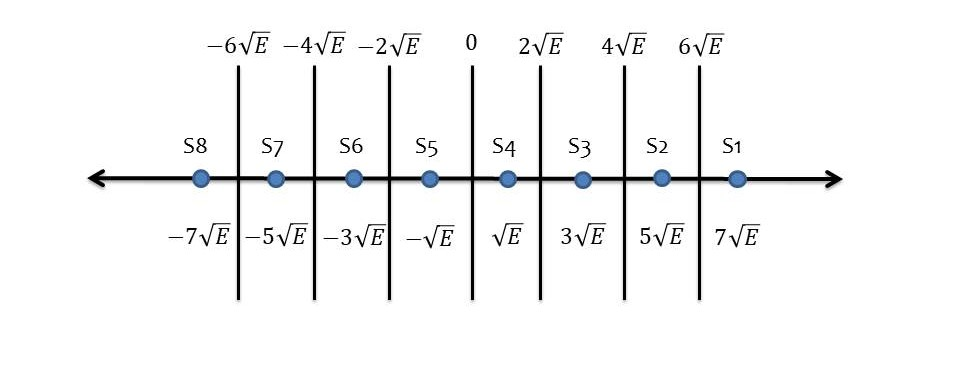
\includegraphics[width=\linewidth]{Figures/Figure_2.jpg}
            \caption{Symbols Boundary}
            \label{fig:Symbols}
        \end{figure}

    \vspace{5cm}

    \subsection{Problem 3}
        The derivation of theoritical bit error rate.
        \begin{equation}
            Pe = \frac{1}{8} \displaystyle\sum_{i=0}^{7} P(e|Si) 
        \end{equation}
        \begin{equation}
            Pe(e|S0) = Pe(e|S7)
        \end{equation}
        \begin{equation}
            Pe(e|S1) = Pe(e|S2) = Pe(e|S3) = Pe(e|S4) = Pe(e|S5) = Pe(e|S6)
        \end{equation}
        Using Union bound S0, S7 only one neighbour and S1, S2,...S6 has two neighbours.
        \begin{equation}
            Pe(e|S0) = \frac{1}{2} erfc(\frac{\sqrt{E}}{\sqrt{N}})
        \end{equation}
        \begin{equation}
            Pe(e|S1) = \frac{1}{2} erfc(\frac{\sqrt{E}}{\sqrt{N}})
                + \frac{1}{2} erfc(\frac{\sqrt{E}}{\sqrt{N}})
        \end{equation}
        \begin{equation}
            Pe(e|S1) = erfc(\frac{\sqrt{E}}{\sqrt{N}})
        \end{equation}
        \begin{equation}
            Pe = \frac{1}{8 * 3} (2 * \frac{1}{2} erfc(\frac{\sqrt{E}}{\sqrt{N}}) 
                + 6 * erfc(\frac{\sqrt{E}}{\sqrt{N}}))
        \end{equation}
        \begin{equation}
            Pe = \frac{7}{24} (erfc(\frac{\sqrt{E}}{\sqrt{N}}))
        \end{equation}

    
    \subsection{Probelm 4}
        \begin{figure}[h!]
            %I put \linewidth into the brackets, which means the picture will be scaled to fit the width of the document.
            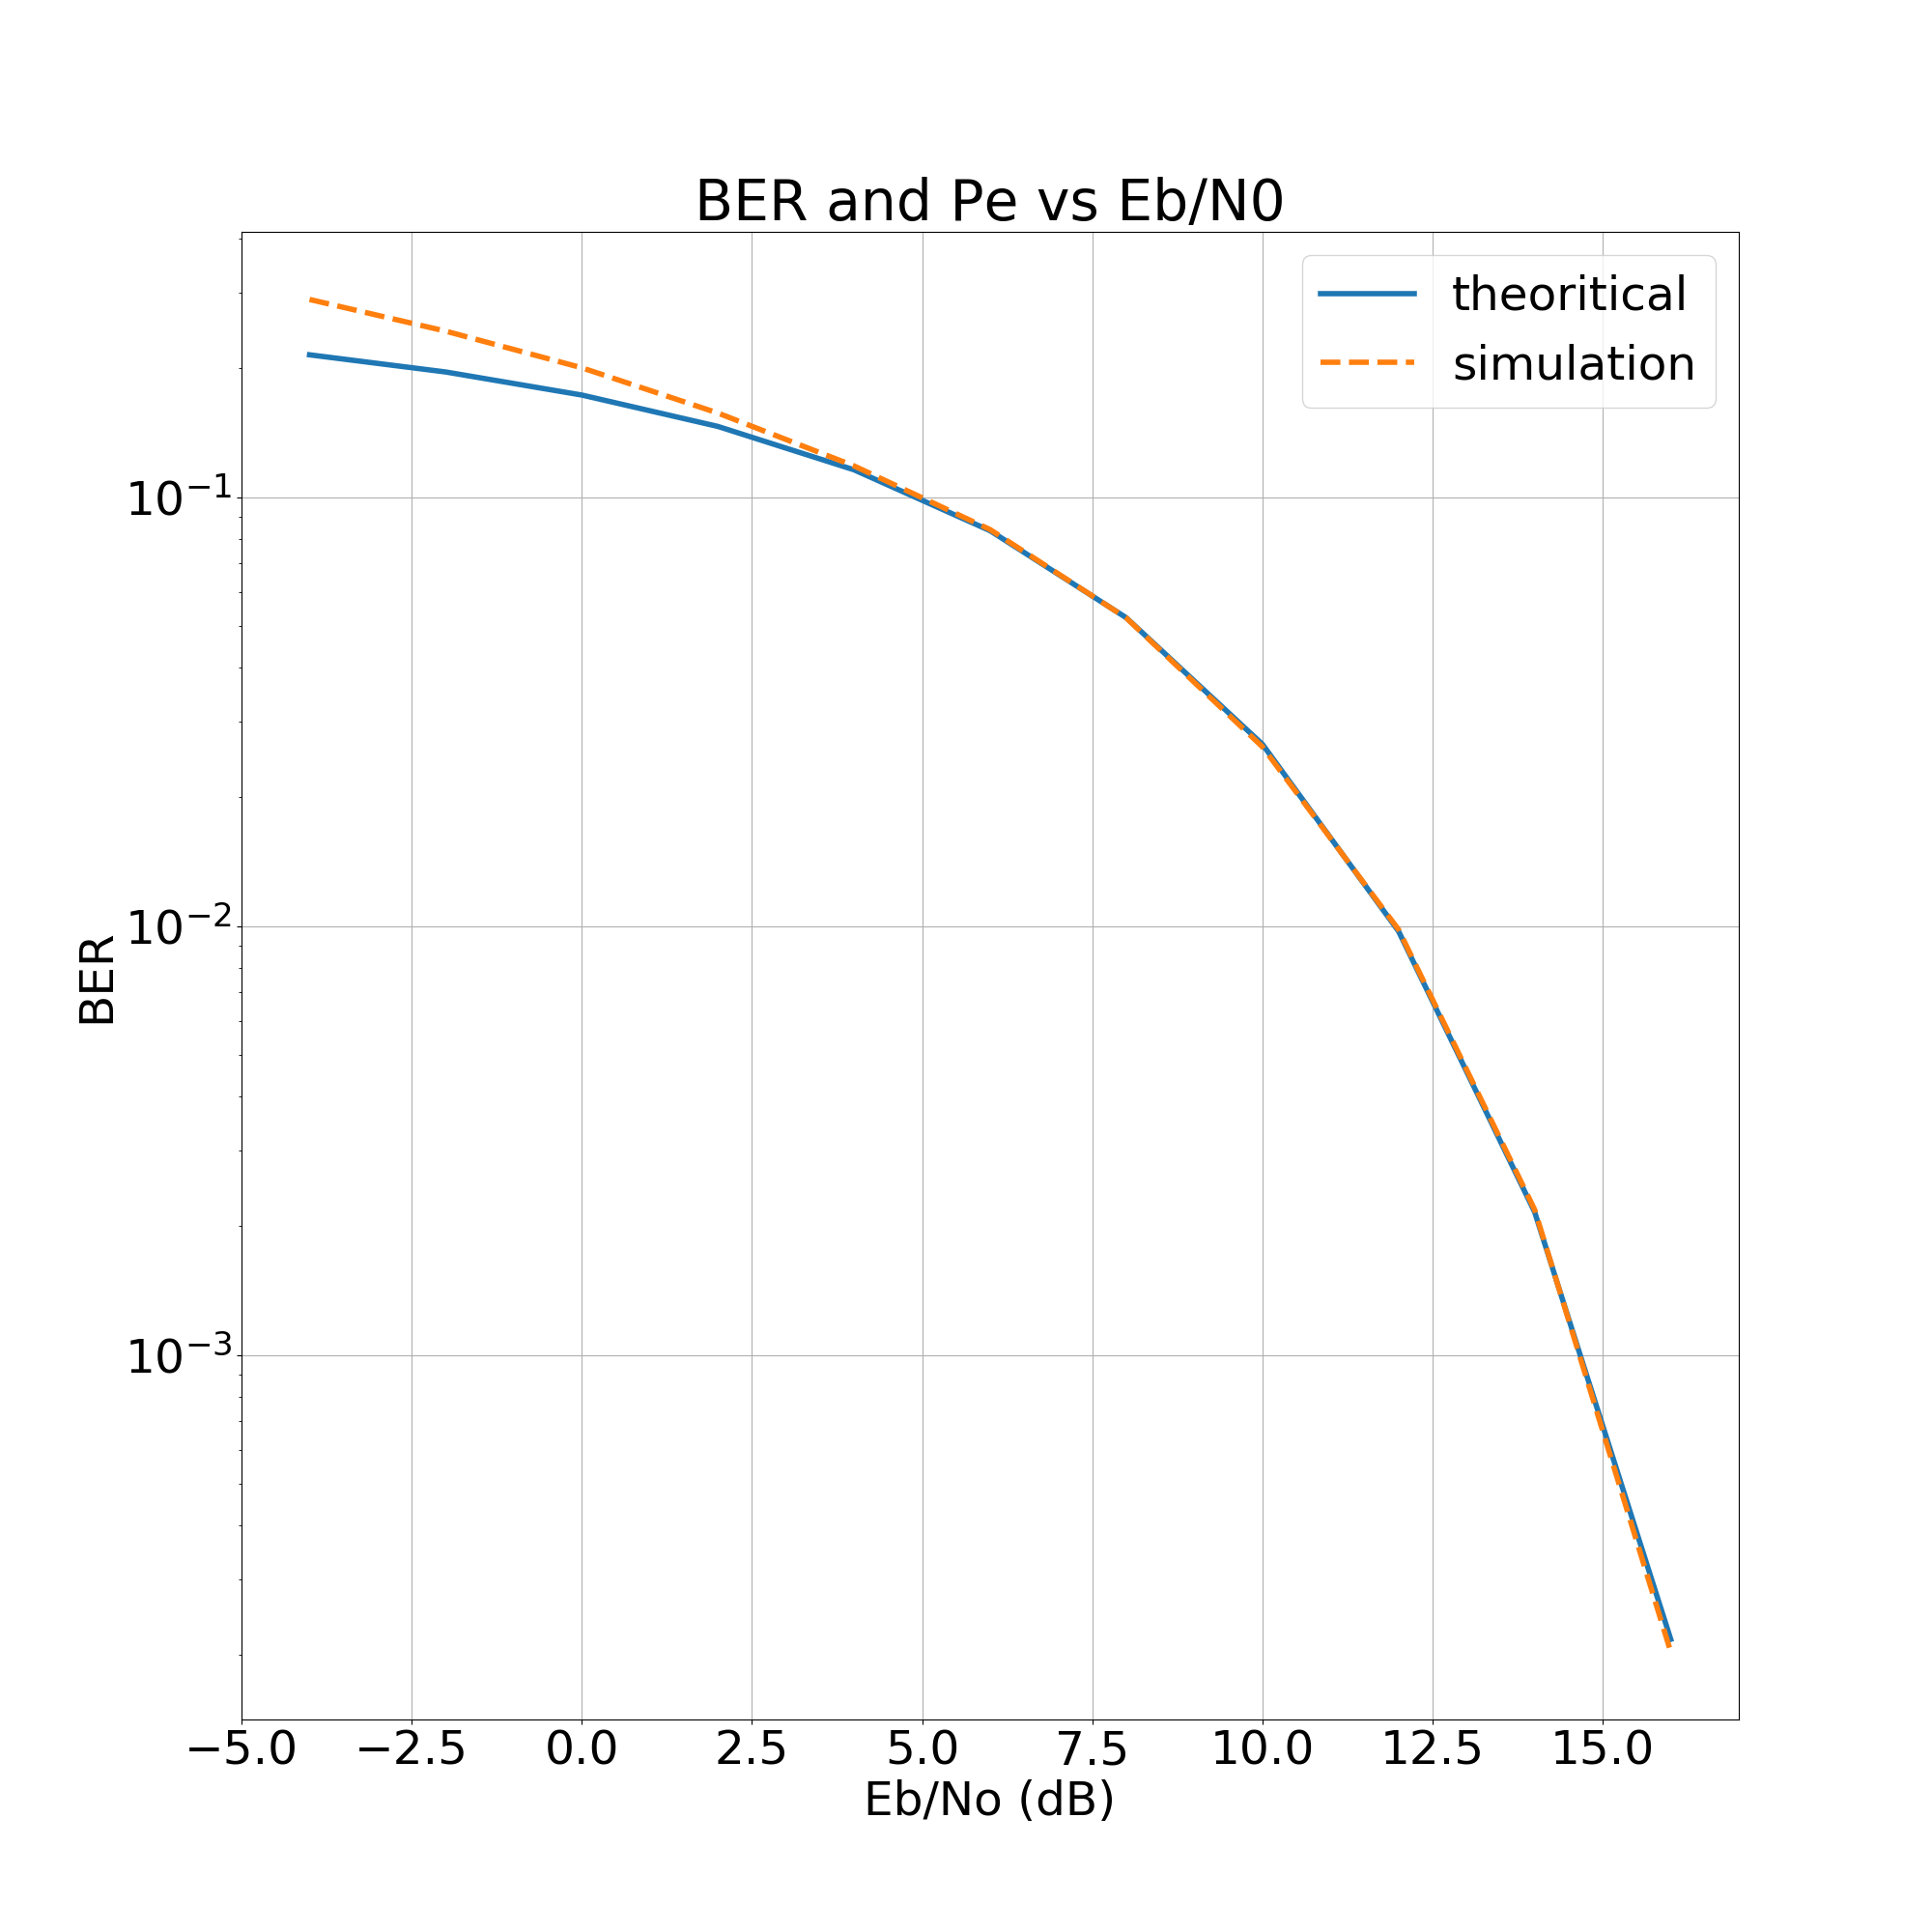
\includegraphics[width=\linewidth]{Figures/Figure_1.png}
            \caption{BER vs Eb/N0}
            \label{fig:BER}
        \end{figure}


    \section{Section 2}
    Hello World 2!

    \subsection{Subsection 2.1}
    Equations:
    %Numbered equation
    
        \begin{equation}
            \frac{n!}{k!(n-k)!} = \binom{n}{k}  
        \end{equation}
        \begin{equation}
            x^\frac{1}{2}  
        \end{equation}
        \begin{equation}
            \frac{\mathrm d}{\mathrm d x} \big( k g(x) \big)
        \end{equation}
    %Unnumbered
        \begin{equation*}
            f(x) = x^2
        \end{equation*}
    
    \section{Math}
    %To write equations withina a sentence
    ...
    This formula $f(x) = x^2$ is an example.
    ...
    \begin{align*}
        f(x) &= x^2\\
        g(x) &= \frac{1}{x}\\
        F(x) &= \int^a_b \frac{1}{3}x^3
      \end{align*}
    
    \section{Figures}
    

    \begin{figure}[h!]
    \centering
    \begin{subfigure}[b]{0.4\linewidth}
        
\includegraphics[width=\linewidth]{slogan.jpg}
        \caption{Meme.}
    \end{subfigure}
    \begin{subfigure}[b]{0.4\linewidth}
        
\includegraphics[width=\linewidth]{slogan.jpg}
        \caption{Same Meme.}
    \end{subfigure}
    \caption{The same meme, Two times.}
    \label{fig:coffee}
    \end{figure}




\end{document}